%%%%%%%%%%%%%%%%%%%%%%%%
%% Sample use of the infthesis class to prepare a thesis. This can be used as 
%% a template to produce your own thesis.
%%
%% The title, abstract and so on are taken from Martin Reddy's csthesis class
%% documentation.
%%
%% MEF, October 2002
%%%%%%%%%%%%%%%%%%%%%%%%

%%%%
%% Load the class. Put any options that you want here (see the documentation
%% for the list of options). The following are samples for each type of
%% thesis:
%%
%% Note: you can also specify any of the following options:
%%  logo: put a University of Edinburgh logo onto the title page
%%  frontabs: put the abstract onto the title page
%%  deptreport: produce a title page that fits into a Computer Science
%%      departmental cover [not sure if this actually works]
%%  singlespacing, fullspacing, doublespacing: choose line spacing
%%  oneside, twoside: specify a one-sided or two-sided thesis
%%  10pt, 11pt, 12pt: choose a font size
%%  centrechapter, leftchapter, rightchapter: alignment of chapter headings
%%  sansheadings, normalheadings: headings and captions in sans-serif
%%      (default) or in the same font as the rest of the thesis
%%  [no]listsintoc: put list of figures/tables in table of contents (default:
%%      not)
%%  romanprepages, plainprepages: number the preliminary pages with Roman
%%      numerals (default) or consecutively with the rest of the thesis
%%  parskip: don't indent paragraphs, put a blank line between instead
%%  abbrevs: define a list of useful abbreviations (see documentation)
%%  draft: produce a single-spaced, double-sided thesis with narrow margins
%%
%% For a PhD thesis -- you must also specify a research institute:
%%\documentclass[phd,ilcc,twoside]{infthesis}

%% For an MPhil thesis -- also needs an institute
% \documentclass[mphil,ianc]{infthesis}

%% MSc by Research, which also needs an institute
% \documentclass[mscres,irr]{infthesis}

%% Taught MSc -- specify a particular degree instead. If none is specified,
%% "MSc in Informatics" is used.
% \documentclass[msc,cogsci]{infthesis}
\documentclass[msc, logo]{infthesis}  % for the MSc in Informatics

%% Master of Informatics (5 year degree)
% \documentclass[minf]{infthesis}

%% Undergraduate project -- specify the degree course and project type
%% separately
% \documentclass[bsc]{infthesis}
% \course{Artificial Intelligence and Psychology}
% \project{Fourth Year Project Report}

%% Put any \usepackage commands you want to use right here; the following is 
%% an example:
\usepackage{natbib}
\usepackage{graphicx}
\usepackage{amsmath}
\usepackage{array}
\usepackage{multirow}
\usepackage[table,xcdraw]{xcolor}
 
%% Information about the title, etc.
\title{ Testing SQL-compliance of current DBMSs}
\author{Elias Spanos}

%% If the year of submission is not the current year, uncomment this line and 
%% specify it here:
% \submityear{1785}

%% Optionally, specify the graduation month and year:
% \graduationdate{February 1786}

%% Specify the abstract here.
\abstract{%
Database Management Systems (DBMSs) are widely used in various fields such as in banking and financial sectors. Hence, the correct and efficient operation of such systems are crucial. As the demand for these systems have been increased rapidly in recent years, different implementations have been proposed and implemented. For example, different companies have been implemented their own system, and inevitably there are significant differences between these systems regarding their internal implementation and architecture. For making easier the transition between these systems a common language was adopted. More precisely, SQL is a database language which is used to manipulate and retrieve data and is supported by all current DBMSs. Albeit different system’s implementations are exist, in principle, they should follow the SQL standards in the same manner. A crucial question that will be investigated by conducting this project is whether DBMSs have been implemented the SQL standards in the same way. The SQL language should pledge that identical SQL code should always return identical answers when it is evaluated on the same database independently of which DBMS is running on. However, there are indications that this is not the case, as SQL standards are interpreted and implemented differently so that identical SQL queries do not always retrieve the same answers.
The aim of this project is the implementation of a random SQL query generator and a comparison tool for investigating and highlighting the differences that may exist among current DBMSs. Further, we aim to provide a detailed explanation in regards to SQL standards of potential differences and explain how they might affect the transition between current DBMSs. 

 
}

%% Now we start with the actual document.
\begin{document}

%% First, the preliminary pages
\begin{preliminary}

%% This creates the title page
\maketitle

%% Acknowledgements
\begin{acknowledgements}
 
I would like to thank my supervisors Paolo Guagliardo and Leonid Libkin who were always willing to advise and help me in order to overcome any difficulty. In addition, I want to thank my family who is always to my side.

\end{acknowledgements}

%% Next we need to have the declaration.
\standarddeclaration

%% Finally, a dedication (this is optional -- uncomment the following line if
%% you want one).
% \dedication{To my mummy.}

%% Create the table of contents
\tableofcontents

%% If you want a list of figures or tables, uncomment the appropriate line(s)
%%\listoffigures
%%\listoftables



\end{preliminary}

%%%%%%%%
%% Include your chapter files here. See the sample chapter file for the basic
%% format.

\include{appendix1}
 
\chapter{Introduction}
 \section{Motivation}


DBMSs are widely used in many fields and find application in many companies as they provide relatively easy way of performing various common operations on data, such as insertion, deletion and update, and at the same time they hide the internal complexity of such  system. More precisely, DBMS is a software that is designed to allow the creation, querying and update of databases [2,3]. The main role of a DBMS is to store and manipulate data efficiently and consistently. Figure 1.1 shows in a high level the structure of modern DBMSs. Additionally, Structured Query language  known as SQL is a standardised programming language for managing relational databases [1]. By having such standards, it can be provided easily a common interface for all DBMSs in order to manipulate and retrieve data from any given database without worrying about the internal implementation. 
 
The aim of this project is to evaluate five systems such as MySQL, IBM DB2, Microsoft SQL Server, PostgreSQL and Oracle Database in order to identify if they interpret the SQL standards in exactly the same way. 

 \begin{figure} 
      \centering
      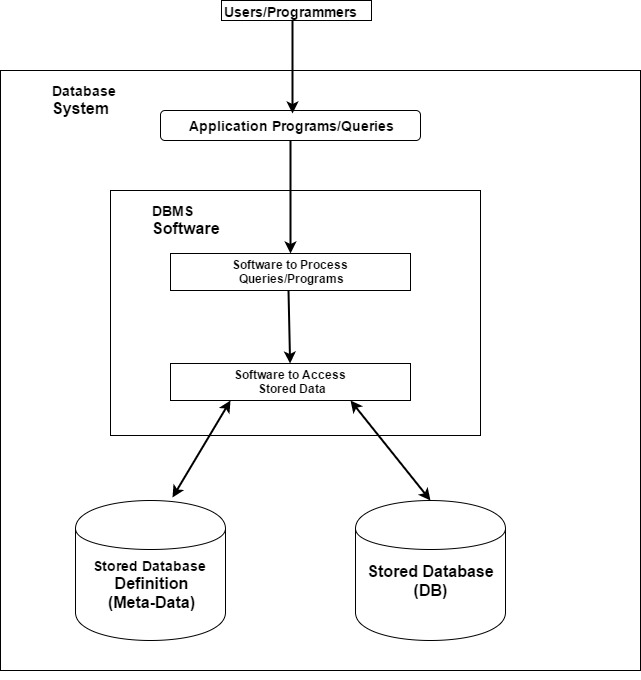
\includegraphics[width=\textwidth]{Images/db_architecture}
      \caption{DBS architecture}
      \label{fig:counting-methods}
    \end{figure}

As it was mentioned all current DBMSs currently support the SQL standards, meaning that there is a common language, namely SQL, that is used by all systems to access, manipulate and retrieve data. Nevertheless some aspects of the standards are not well defined which make the process of interpret and implement it a difficult task and as a results, companies implement the SQL standards in a different manner. As a consequence programs that are written in SQL are partially portable among different DBMS.  



\begin{table}[h]
\centering
\caption{My caption}
\label{my-label}
\begin{tabular}{lll}
\multicolumn{3}{l}{\textbf{Is it a bug?}}                                                                               \\
                                       & \multicolumn{1}{c}{\textbf{Y}}           & \multicolumn{1}{c}{\textbf{N}}      \\ \cline{2-3} 
\multicolumn{1}{l|}{\textbf{Bugs}}     & \multicolumn{1}{l|}{True Positive (TP)}  & \multicolumn{1}{l|}{False positive} \\ \cline{2-3} 
\multicolumn{1}{l|}{\textbf{Reported}} & \multicolumn{1}{l|}{False Negative (FN)} & \multicolumn{1}{l|}{True Negative}  \\ \cline{2-3} 
                                       &                                          &                                    
\end{tabular}
\end{table}


\begin{math}
\frac{2}{3}
\end{math}

\chapter{Background}

\section{The SQL Standard }
DBMS from its first appearance shows that it will be the dominant trend for managing data. Consequently, different implementations have been emerged from various vendors and inevitable, a standardized language should be implemented in order to provide portability among different systems. If applications were implemented using only SQL commands which are defined in that standard and vendors implemented these commands in exactly the same way, then SQL code could be migrated on any DBMS without the need to be adopted. As it was mentioned, the common language for relational database management system (RDMS) is SQL. 

The first appearance of the SQL language was in 1970 where IBM developed the first prototype of RDMS. Subsequently, the first SQL standard arose in 1986 by American National Standard Institute (ANSI) with the name SQL-86 for bearing conformity among vendors’ implementations. Since then different flavors of the standard have being emerged for revising previous versions or for adding new features such as SQL-87, SQL-89, ANSI/ISO SQL-92 and  ANSI/ISO SQL: 1999 which has been approved also by International Standards Organization (ISO) [11]. SQL standard has been continuously developed with current version being SQL:2016 or ISO/IEC 9075:2016. The ANSI SQL standard is divided into several parts and this project focus on the SQL/Foundation part. This part contains central elements of SQL. Explanations about the findings are explained according to SQL:2016 since it is the newest version of the standard, though this parts  remains the same in comparison with earlier flavors. 

\section{The SQL Language}
SQL operations are in the form of commands known as SQL statements. More precisely, SQL is consisted primarily by two sublanguages such as data definition language (DDL) and data manipulation language (DML). DDL is a part of SQL language and can be used to create, modify, delete tables and views, and usually DDL statements start with keywords CREATE, DROP and ALTER. Also, it supports a command that give the capability to be defined new domains. Moreover, in general tables and rows are denoted as relations and tuples and sometimes it referred to these terminologies. DML is also a part of the SQL language that is consisted by a family of commands like any programming language and is used for the creation of a query for inserting, modifying and deleting rows in a Database. This sublanguage is consisted by SELECT-FROM-WHERE commands as to be the fundamental for any query. In addition, SQL standard supports more complex rather than just these simple commands for performing various tasks on data. For example, aggregation functions such as Sum, Max, Min, Avg are used with combination with Group By, and Having SQL statements. The purpose of having such commands is to perform a calculation on a specific  columns in order to return a value. An example can be if we want to calculate the average salary of a department. Then, we need to perform a group by based on all the salaries of the employees of that department. 
Hence, SQL is extremely popular as it offers two capabilities. Firstly, it can access many tuples using just one command and secondly it does not need to specify how to reach a tuple, for example by using an index or not. 

\section{Commands of SQL}

This subsection intends to introduce in a high-level overview the basic commands of SQL which are defined in the SQL standard and it is described briefly the usefulness of each command. As some these commands are used to generate random SQL queries, it is important to provide a basic background of the usage and purpose of each command. 

\noindent\textbf{\underline{SQL Basic Structure}} 
\begin{mdframed}[backgroundcolor=gray!20] 
\begin{lstlisting}
SELECT [DISTINCT] columns_list
FROM tables_list
WHERE Condition1 {AND|OR} Condition 2
\end{lstlisting}
\end{mdframed}
The SQL basic structure is used to retrieve data from a database according to some criterias which are specified in the WHERE clause. Each SQL query should contain at least SELECT and FROM clause and an optional WHERE clause. The main idea of the basic SQL query is to go through all the rows of the tables listed in the FROM Clause, and each row that satisfied the search criteria is selected. Then, only the specified columns of the selected rows are appear in the result. The DISTINCT keyword is optional and it is used to eliminate duplicates rows in the result. Also, instead of having columns\_list in the SELECT clause, it can be used the “\*” keyword which indicates that all the columns will be appeared in the result. Different conditions can appear in the WHERE clause using logical connectivities such as AND, NOT and OR.  

\noindent\textbf{\underline{Example:}}
\begin{mdframed}[backgroundcolor=gray!20] 
\begin{lstlisting}
SELECT St.Student_Name
FROM Students AS St 
WHERE St.age >= 20 AND St.age <= 24
\end{lstlisting}
\end{mdframed}

The above example uses the basic SQL structure to build a query. Thus, it returns all the name of students who are between 20 and 24 year old. 

\noindent\textbf{\underline{SQL Basic aggregation Syntax:} }
\begin{mdframed}[backgroundcolor=gray!20] 
\begin{lstlisting}
SELECT       [DISTINCT]  Columns_list
FROM         Tables_list
WHERE        Condition1 {AND|OR} Condition2
GROUP BY     Columns_list
HAVING       Condition1 {AND|OR} Condition 2
\end{lstlisting}
\end{mdframed}

Queries with aggregation have as goal to perform a calculation on a specific columns in order to return a value. GROUP BY and HAVING are used to perform an aggregation. HAVING is an optional clause, and aggregation can be still perform using aggregate commands in the SELECT clause. A concrete example is given subsequently. 

\begin{table}[h]
\centering
\caption{My caption}
\label{my-label}
\begin{tabular}{|l|l|}
\hline
\multicolumn{2}{|l|}{\textbf{Aggregate Commands}}                                                             \\ \hline
\textbf{Command}                        & \textbf{Usage}                                                      \\ \hline
{\color[HTML]{333333} \textbf{MIN()}}   & {\color[HTML]{333333} Finds the minimum value,of a column}          \\ \hline
{\color[HTML]{333333} \textbf{COUNT()}} & {\color[HTML]{333333} Counts the total number,of rows}              \\ \hline
{\color[HTML]{333333} \textbf{MAX()}}   & {\color[HTML]{333333} Finds the maximum value,of a column}          \\ \hline
{\color[HTML]{333333} \textbf{SUM()}}   & {\color[HTML]{333333} Calculates the sum of,values of a column}     \\ \hline
{\color[HTML]{333333} \textbf{AVG()}}   & {\color[HTML]{333333} Calculates the average of,values of a column} \\ \hline
\end{tabular}
\end{table}


Aggregate commands can be used both in SELECT and HAVING Clause with a combination with the existence of GROUP BY clause in the SQL query. The below example illustrates the proper use of aggregate commands.


\noindent\textbf{\underline{Example: :} }
\begin{mdframed}[backgroundcolor=gray!20] 
\begin{lstlisting}
SELECT COUNT(St.student_id), St.Country
FROM Students AS St 
GROUP BY St.Students
HAVING COUNT(St.student_id)  >  3
\end{lstlisting}
\end{mdframed}

The above query makes proper uses of the aggregation commands. The concrete query list the number of students in each country where there are more than three students in a specific Country. 

 
\begin{table}[h]
\centering
\caption{My caption}
\label{my-label}
\begin{tabular}{|l|l|}
\hline
\multicolumn{2}{|l|}{\textbf{Commands}}                                                                                                \\ \hline
\textbf{Command}                       & \textbf{Usage}                                                                                \\ \hline
{\color[HTML]{333333} \textbf{EXISTS}} & {\color[HTML]{333333} Returns true if there is,at least one row in the subquery}              \\ \hline
{\color[HTML]{333333} \textbf{Op ALL}} & {\color[HTML]{333333} Returns true if all the,comparisons using an operator OP are true}      \\ \hline
{\color[HTML]{333333} \textbf{Op ANY}} & {\color[HTML]{333333} Returns true if at least,one comparison using an operator returns true} \\ \hline
{\color[HTML]{333333} \textbf{Op IN}}  & {\color[HTML]{333333} Returns true if an,element exist in a given set}                        \\ \hline
{\color[HTML]{333333} \textbf{LIKE}}   & {\color[HTML]{333333} Returns true if an,attribute matches with a pattern}                    \\ \hline
\end{tabular}
\end{table}



\noindent\textbf{\underline{Example: :} }
\begin{mdframed}[backgroundcolor=gray!20] 
\begin{lstlisting}
SELECT *
FROM Students AS St 
WHERE St.Country IN (‘UK’, ‘Netherland’)
\end{lstlisting}
\end{mdframed}
The above query retrieves all the students who come from UK, Cyprus and Netherland.

 
\begin{table}[h]
\centering
\caption{My caption}
\label{my-label}
\begin{tabular}{|l|l|}
\hline
\multicolumn{2}{|l|}{\textbf{SET Commands}}                                                                                                                                \\ \hline
\textbf{Command}                                    & \textbf{Usage}                                                                                                       \\ \hline
{\color[HTML]{333333} \textbf{UNION {[}ALL{]}}}     & {\color[HTML]{333333} Returns the combination,of the results of two SQL queries}                                     \\ \hline
{\color[HTML]{333333} \textbf{INTERSECT {[}ALL{]}}} & {\color[HTML]{333333} Return the combination of,the results of two SQL queries for rows that,appear in both,results} \\ \hline
{\color[HTML]{333333} \textbf{EXCEPT {[}ALL{]}}}    & {\color[HTML]{333333} Return each row that,appear to the first query but does not appear to the second query}        \\ \hline
\end{tabular}
\end{table}

By default SET commands remove duplicates in the SQL result. Nevertheless, if it is needed to have duplicates in the result then the ‘ALL’ keyword is used.  


\noindent\textbf{\underline{Example: :} } 
\begin{mdframed}[backgroundcolor=gray!20][h]
\begin{lstlisting}
SELECT Country FROM Students 
UNION
SELECT Country  FROM  Professor
\end{lstlisting}
\end{mdframed}

The above query retrieves the Countries where there both Students and professors. 

 
\begin{table}[]
\centering
\caption{My caption}
\label{my-label}
\begin{tabular}{|l|l|}
\hline
\multicolumn{2}{|l|}{\textbf{String Commands}}                                                                            \\ \hline
\textbf{Command}                          & \textbf{Usage}                                                                \\ \hline
{\color[HTML]{333333} \textbf{TRIM()}}    & {\color[HTML]{333333} Returns the string,without leading/trailing characters} \\ \hline
{\color[HTML]{333333} \textbf{CONCAT()}}  & {\color[HTML]{333333} Concatenate two or more,strings}                        \\ \hline
{\color[HTML]{333333} \textbf{REPLACE()}} & {\color[HTML]{333333} Replaces a subset of a,string with another string}      \\ \hline
\end{tabular}
\end{table}


\noindent\textbf{\underline{Example: :} }
\begin{mdframed}[backgroundcolor=gray!20][h]
\begin{lstlisting}
SELECT SUBSTRING (“SQLSTANDARD”, 1, 3 ) AS SQLExtraction  
\end{lstlisting}
\end{mdframed}

The above SQL query extract from the string which is given as parameter to the SUBSTRING function the first three characters starting from the position 1. Thus, the results is: “SQL”

\begin{table}[h]
\centering
\caption{My caption}
\label{my-label}
\begin{tabular}{ll}
\hline
\multicolumn{2}{|l|}{\textbf{Data Types}}                                                                                                                                      \\ \hline
\multicolumn{1}{|l|}{\textbf{Types}}                           & \multicolumn{1}{l|}{\textbf{Description}}                                                                     \\ \hline
\multicolumn{1}{|l|}{{\color[HTML]{333333} \textbf{SMALLINT}}} & \multicolumn{1}{l|}{{\color[HTML]{333333} Returns the string,without leading/trailing characters}}            \\ \hline
\multicolumn{1}{|l|}{{\color[HTML]{333333} \textbf{INT}}}      & \multicolumn{1}{l|}{{\color[HTML]{333333} Concatenate two or more,strings}}                                   \\ \hline
\multicolumn{1}{|l|}{{\color[HTML]{333333} \textbf{BIGINT}}}   & \multicolumn{1}{l|}{{\color[HTML]{333333} Replaces a subset of a,string with another string}}                 \\ \hline
\multicolumn{1}{|l|}{\textbf{VARCHAR}}                         & \multicolumn{1}{l|}{Takes as input the length,of a variable string which can contains up to 255 characters}   \\ \hline
\multicolumn{1}{|l|}{\textbf{CHAR}}                            & \multicolumn{1}{l|}{Takes as input the length,of a fixed size string which can contains up to 255 characters} \\ \hline
                                                               &                                                                                                              
\end{tabular}
\end{table}

\subsection{Missing values} 

This section aims to provide a basic background regarding NULLs and introduce the problems that can be arised from having NULLs in a DBMS. In the section of experiments, it is illustrated that many problems can be appeared by using NULLs. SQL uses NULL marker for missing or unknown values in a database and for that reason NULL is a reserved word. It worthy mentioning that NULL should not be confused with a value of zero or an empty string. Nevertheless, Oracle treats the empty string as NULL [12].  An important consideration is that it cannot be tested if a value of a field is NULL using usual comparison operators such as $ <>, = $ and $<$ but instead IS NOT NULL and IS NULL commands are used. In general the existence of NULL is the fundamental source of issues and incompatibilities among current DBMS. For evaluating each comparison with the existence of NULLS a three-valued logic (3VL) is proposed which is an extension of common boolean logic. In boolean logic, there are two values that an expression can be evaluated, namely, TRUE AND FALSE, where the negation evaluate to the opposite values. On the contrary with 3VL, in 3VL there is an addition value called unknown and the opposite of it remains the same. In addition, all comparisons involving NULL should be resulted to be unknown according to SQL Standard. Below it is illustrated a truth table for the different comparisons with the suitable outcomes.    

\subsection{SQL standard issues} 

Below it is provided a few concrete examples which demonstrate that indeed some aspects of the Standard is implemented differently by each vendor. 
 
\noindent\textbf{Example:}

For example the SQL query below does not return identical results on both PostgreSQL and Oracle [14]. 


\begin{mdframed}[backgroundcolor=gray!20][h] 
Q1:SELECT * 
 \\FROM ( SELECT S.A, S.A FROM S ) R
\end{mdframed}

While it is expected Q1 to return identical results independently on which systems is executed on, this is not the case. It can be observed that Q1 will output a table with two columns named “A” in PostgreSQL. On the other hand, in Oracle database, the SQL query will return an compile-time error. Ιndisputably, there are differences between current DBMSs [1]. 
It can supposed that in most of the cases these differences are minor but if we take into account that these systems are used in many different fields, then we can quickly realise that small differences might be critical. The key idea is to be conducted an experimental evaluation of current DBMSs. 






\chapter{Methodology}

\section{Methodology}
 
In this chapter will be describe the main strategy that will be used in order to test the SQL compliance of current DBMSs. 

 As it was mention, the key idea of the current project is to examine whether current DBMSs respect the SQL standards and to highlight the differences that might exist among those systems. One of the core component that will be used  for testing the SQL compliance is the Random SQL Generator tool. Thus, the first goal is to design and implement such a tool which will generate a diversity of SQL queries by exposing the expressivity of SQL language. It is worthy mentioning that this tool can be important of its own use by utilize it for testing a new DBMSs. The implementation of the tool will be in such a way that a new DBMS can be added without affect almost anything of the current implementation. A detailed explanation about the implementation and the internal structure of the tool is given in the following Chapter. Additionally, by having such a tool, it will be possible to generate thousands of different SQL queries and evaluate them in five systems, namely PostgreSQL, Microsoft SQL Server, IBM DB2, Oracle Database and MySQL for identifying differences. 
Subsequently, another useful tool that it will be designed and implemented is the run and compare tool. Apparently this tool must be compatible with all the DBMSs and it should evaluate each query and compare the results of each DBMS whether they are identical with concerning the rest systems. The comparison of DBMS’s results will be performed using main-memory data structure for achieving efficiency. In case where a difference between any system will be found, then a log file will be created to record all the differences. Again a detailed explanation of tool’s internal implementation is given in the next chapter.
Lastly but not least, a tool is needed for generating random data in order to perform our experiments. For that purpose, datafiller will be used which is a well-known open-source tool that provides the capability of generating realistic data. The data are generated based on a database schema which is provided to the tools as a parameter and many parameters can be specified for generating realistic data with different sizes. 







 
\chapter{Implementation}
In this chapter we describe in details the framework that we implemented for testing the SQL-compliance for current DBMSs.


\section{Implementation}
The framework is composed by different tools such as random SQL generator engine, comparison tool and random data generator.  All tools are implemented in Java programming language which can run on all platforms that support Java except the random data generator which we use an open source python script that can generate realistic datasets.

 \begin{figure} 
      \centering
      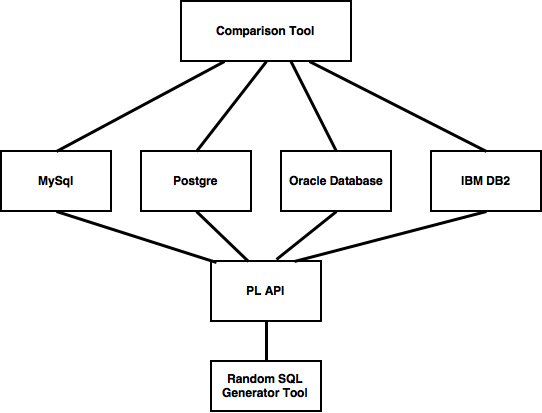
\includegraphics[width=\textwidth]{Images/Chapter4/1-implemen_detail}
      \caption{Random SQL Generator Architecture}
      \label{fig:counting-methods}
    \end{figure}


\subsubsection{Random SQL generator engine}
One of the most important components of the framework is the random SQL generator tool which can be used to generate thousand of different queries for evaluating the current DBMSs. Obviously SQL language has a strong power expressivity and as a consequence it supports many commands where some of them are simple in terms of their use such as SELECT, FROM, WHERE and some other more trickier such as GROUP BY, HAVING or aggregation functions where we need to care about the proper use of these commands and generating syntactically correct SQL queries. As a result, for achieving that our implementation is composed by various classes where each of them is used for different purpose. It is worthy mentioning that the tool can be used by its own use for other purposes. Thus, in this work, we have designed and implemented this tool from scratch using Java programming language. In addition, the tool has been designed in a way that it is modular and reusable for supporting new DBMSs in the future without the need of changing the whole structure of the tool. Thus, the main idea of the tool is to generate a diversity of queries for testing the DBMSs.  
The random SQL generator tool is consisted by different Java classes and a configuration file. An important consideration was how to design our generator tool in a way that will be feasible to generate different valid SQL queries and at the same time to be syntactically correct. Hence, we have implemented an internal representation for generating randomly SQL queries and each class is responsible for generating a different statement  that contribute to the overall query. For example, one of the classes that constitutes the tool is the SELECT class which obviously this class is responsible for generating the SELECT clause of each SQL query. Having different classes for each clause, it makes it easier to extend the tool in order to add new functionality and at the same time there is no need to change other part of the code. The final SQL query is converted to an SQL string and is executed to the current DBMSs. It is not feasible to generate SQL strings directly because we need to track things. If we generating just strings, it will not possible to check if in the WHERE clause it is mentioning attributes that appear in the FROM clause or they comes as parameters from the outer query. Thus, there is a need to track attributes for each clause. 
Another important consideration that we had to think about was how to avoid generating completely random SQL queries. Even though we need to generate random SQL queries to stress the existing DBMSs in different situations, we need to control some characteristics of the SQL query. For example, imagine an SQL query that performs a cartesian product with a large number of tables. In this situation, we will have as a consequence the query to be executed for a long time or even for ever and it is not so useful for our goal. Many parameters can be specified from the configuration file such as maximum level of nesting, max number of tables in a FROM, probability of having arithmetic comparisons. More details about the configuration file is given subsequently. As a consequence, our tool supports a configuration file that can be used to control the randomly generated SQL queries. Below is provided a part of the configuration file and some of the main parameters are explained.     

It can be seen from the configuration file that we can control many parameters, nevertheless it does not imply that we restrict the diversity of SQL query that can be generated. For example, we can set an upper bound of tables that appear in the FROM clause. In that way, we avoid having an enormous table size from cartesian product. In addition, even it is not so usual to have constant comparison in an SQL query, nevertheless SQL standards support this. Thus, we generate SQL queries which have constant comparisons but we do not need to have a lot of such queries. An example of such query is as follow:

SELECT r41.A AS A0
FROM r4 AS r41
WHERE 1 > 2

We can specify the probability of having such cases by setting the parameter probWhrConst which have a domain between 0 and 1 meaning that if the value is 1 then there will be exist for sure a constant comparison.
	Another important parameter which can be specified from the configuration file is the level of nesting. We can randomly generate SQL queries with a specific level of nesting. The example below demonstrates a query with level of nesting three. For generating such a query many consideration should be taken into account. For example, we should track attributes for outer queries, as inner query can access outer attributes or attributes from its FROM clause. The opposite is not true, meaning that we cannot access attributes from an inner query. 





SELECT r12.A AS A0, r12.B AS A1, r22.A AS A2 
FROM r1 AS r12, r2 AS r22
WHERE NOT(NULL <> 9 OR r12.A >= r22.A OR ( NOT(5 > 3 )  ) 
AND r12.A = ANY( (	SELECT r43.B AS A0
			FROM r4 AS r43, r1 AS r13, r2 AS r23
			WHERE (NULL >= 3)AND r22.B IN (SELECT r43.A AS A0
							FROM r4 AS r44, r2 AS r24
							WHERE (15 < 2 AND NOT(NULL >= 14 ) ) 



	Another important decision that should be taken into account is how we can provide the relations and attributes to the tool. An initial approach was to be given as parameters in the configuration file. Albeit this approach works pretty well, it makes our tool not portable. Image if the DBMSs have lots of tables with many columns. Hence, It will be time-consuming to give these parameters via the configuration files. Thus, an efficient approach is to retrieve the whole schema from DBMSs automatically. As a result, our tool has the capability to automatically retrieve the whole schema for any DBMS just by providing the credential for connecting to the database in the configuration file.

\section{Comparison Tool} 
As it was mentioned the purpose of the random query generator tool is to generate thousand of SQL queries which can be then used to evaluate current DBMSs. The result of each query can be huge in terms of its cardinality with different order. As a consequence, there was a need to automate the process and identify any difference that may exist by comparing the results efficiently. Therefore, we illustrate below our comparison tool (CT) which has been implemented for achieving the aforementioned goal and further we provide a detailed explanation about the internal implementation of the tool.  

 \begin{figure} 
      \centering
      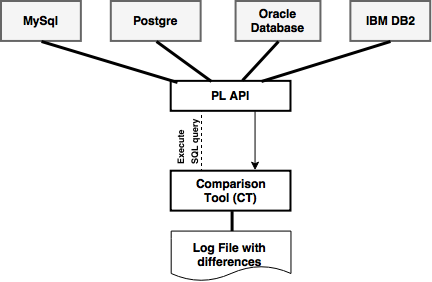
\includegraphics[width=\textwidth]{Images/Chapter4/2-ComparisonTool}
      \caption{Simple Architecture of Comparison Tool}
      \label{fig:counting-methods}
  \end{figure}

We have implemented the CT in Java programming language in order to compare the output results of each DBMSs. The tool is an important component of our project as it is used to conduct our experiments and identify the main differences that exist between current DBMSs. Apparently, differences may be minor or extremely difficult to be identified as DBMSs try to follow the SQL standards. Nevertheless, we illustrate in our experiments that differences exist and in some of the cases may be significant depends on the context that DBMSs are used. Comparing the results of each SQL query is not an easy task because each DBMSs use different algorithms to evaluate them and they return the output results in different order or their output format differ. The CT is fully compatible with the random generator engine and it takes as input each SQL query which is generated by the random SQL generator and subsequently evaluates each query to the current DBMSs. As a result, we use a data structure, namely LinkedList to store each row and then we use an efficient in-memory sorting algorithm to sort the rows. Then, we compare each rows of each DBMS and check if any row differ or does not exist. In case where the results are not identical, a log file is generated and we record which DBMSs differ and what is the SQL query that cause the problem.

 \begin{figure} 
      \centering
      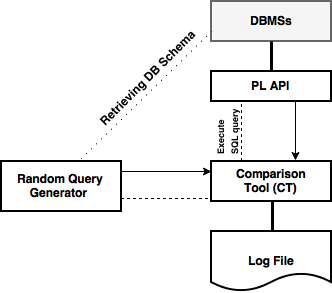
\includegraphics[width=\textwidth]{Images/Chapter4/3-ComparisonTool}
      \caption{Architecture of Comparison Tool}
      \label{fig:counting-methods}
  \end{figure}


\section{Generate data}
Datafiller is a well-known open-source project that provides the capability of generating random data. Thus it will be used in this project for generating a diversity of  data sets in order to evaluate all major DBMSs. More precisely, the datafiller script generates random data, based on a data schema which is given as a parameter, and by taking into account constraints of that schema. For example, it takes into account the domain of each field and if the field should be unique, foreign key or primary key. Another important parameter is the df: null=x.xx% which indicated nullable rates. It will be extremely useful to test the behaviour of current DBMS in a database with nulls and check if there are differences.     

Additionally, more complex parameters can be provided as well, such as a number of tuples per table using --size SIZE parameter. It worthy mentioning that these parameters should be defined within the schema script and should start with -- df.  Further, we can generate more realistic data by providing some information in the schema script of the database. For example, if we have a field that represents a date, then we can provide a specific range in order for the datafiller to generate dates only within this range. This can be achieved by specifying the following parameter: range -- df: start=year-month-day end=year-month-day beside the date field. Subsequently, we need to add the --filter parameter while running the script. These are only some of the important parameters that the datafiller provides but apart from these, it provides more sophisticated properties which are out of importance for our project.

It is important mentioning that the datafiller does not support importing data to other databases such as Oracle database, MS Server or IBM DB2 except postgresSQL. As a result, our approach is to import the data in postgreSQL and then export the random generated data in a CSV files. In this way, we can import the CSV files in all the DBMS, as all of them support importing data from CSV files.  


\chapter{Experimental Evaluation}
This chapter presents the procedure that it is followed in order to provide the experimental evidences. Subsequently, It is presented the main findings with appropriate explanation according to the Standard. Also, it is described  the environment and the DBMSs that they have been tested. 

\section{The experiment Set-Up}
The evaluation is carried out on Windows 8 with i7 CPU, 12GB Ram and a solid state disk (SSD). Also, the  following versions of DBMSs have been installed: PostgreSQL Version 9.6, Microsoft SQL Server Express Edition 2016, IBM Db2 Express-C, Oracle Database 12c and  MySQL Community Edition 5.7. 
Apart of generating huge numbers of SQL queries, it is also checked if new findings can be emerged by conducting the experiments in different schemas with different data types and numbers of relations. As a result, it is checked the following data types:  TEXT, CHAR, VARCHAR, INTEGER, SMALLINT, BIGINT. Moreover, the experiments are conducted in different schemas varying from two to ten relations with two to ten attributes. In addition, it is generated data using different rate of NULLs such as 5%, 10%, 20% and 40% for identify if differences can arise depending on the number of NULLs that a database contains.  Furthermore, the size of instances varied from two to one thousand rows which were generating using data fiiller. Having huge instances decrease the throughput of queries that can be executed per second and thus less queries will be checked. Taking into account that issues and different interpretations can be raised even in small instances, it is end up realized that small instances and schema can still reveal crucial differences. 

\section{Experiment Results}
The implemented architecture is used to conduct the experiments and in that way it is also checked whether the current implementation if is capable to detect any differences among modern DBMSs. The results are provided below with the following format: Firstly,  It is presented  the SQL query that cause an error or a semantic issue on one or more systems. Meaning that some features may not be implemented by all systems or use a different commands or interpret it differently.  Then, a table for each query is provided that demonstrates a raised error of any system, otherwise, the keyword ‘works’ meaning that the SQL query is executed without to raise any error. Thereafter, a comprehensive explanation is given for each problematic query by explaining about the source of the problem and giving an explanation according to the SQL standard.   

\subsection{Dif 1}

\textbf{Q1:}
\begin{mdframed}[nobreak=true, backgroundcolor=lightgray!20] 
\begin{lstlisting}[style=SQL]
SELECT r41.A AS A0
FROM r4 AS r41
WHERE 1*1
\end{lstlisting}
\end{mdframed}

\begin{table}[h]
\centering
\caption{Difference 1}
\begin{tabular}{|p{2cm}|p{11.5cm}| }
\hline
\textbf{DBMS} & \textbf{Result Message}                                                                                                 \\ \hline
Mysql         & Works                                                                                                                   \\ \hline
PostgreSQL    & {[}42804{]} ERROR: argument of WHERE must be type boolean, not type integer                                             \\ \hline
MS Server     & {[}S0001{]}{[}4145{]} An expression of non-boolean type specified in a context where a condition is expected, near '1'. \\ \hline
Oracle        & {[}42000{]}{[}933{]} ORA-00933: SQL command not properly ended                                                          \\ \hline
IBM DB2       & Works                                                                                                                   \\ \hline
\end{tabular}
\end{table}

According to SQL standard each expression in the WHERE clause should be evaluated to a boolean type such as True or False. Thus, DBMSs evaluate each row based on the SQL query and if the WHERE clause is evaluated to True, then the specific row appears in the output results. We expect that arithmetic comparisons between two numbers should return an integer type instead of boolean type. Thus, if the query 1 is executed on any DBMSs should raise an error. Nevertheless, Mysql and IBM DB2 execute the query without to raise any error even though there is an arithmetic comparison  in the WHERE clause such as 1*1. Albeit expressions in the WHERE clause should return a boolean type, these two DBMSs convert arithmetic comparison into a boolean type. On the contrary, the rest three DBMSs throw an exception while they executing the query which is something reasonable as they expect a boolean type in the WHERE Clause. 

\subsection{Dif 2}
  
\textbf{Q2:}
\begin{mdframed}[backgroundcolor=lightgray!20] 
\begin{lstlisting}[style=SQL]
SELECT r21.A AS A0 
FROM r2 AS r21
WHERE true
\end{lstlisting}
\end{mdframed}
 
 
\begin{table}[h]
\centering
\caption{Difference 2}
\label{my-label}
\begin{tabular}{|p{2cm}|p{11.5cm}| }
\hline
\textbf{DBMS} & \textbf{Result Message}                                                                                                   \\ \hline
Mysql         & Works                                                                                                                     \\ \hline
PostgreSQL    & Works                                                                                                                     \\ \hline
MS Server     & {[}S0001{]}{[}4145{]} An expression of non-boolean type specified in a context where a condition is expected, near 'true' \\ \hline
Oracle        & {[}42000{]}{[}920{]} ORA-00920: invalid relational operator                                                               \\ \hline
IBM DB2       & Works                                                                                                                     \\ \hline
\end{tabular}
\end{table}

As it was mentioned before each expression in the WHERE clause is evaluated to true or false. Thus, instead of having an expression, it can be specified the true/false keyword which is a boolean type. As a consequence, it will be reasonable to have the ‘true’ keyword in the WHERE clause meaning that each row will be included in the results. Nevertheless, not all the DBMSs support this. MS server and Oracle do not support this keyword. With respect to SQL standard there is not explicit mention about the keyword true in the WHERE Clause. 

\hfill\newpage
\subsection{Dif 3}

\textbf{Q3:}
\begin{mdframed}[backgroundcolor=lightgray!20]
\begin{lstlisting}[style=SQL]
SELECT  NULL/NULL, 1/2, NULL-NULL
FROM r2 AS  r21, r4  AS  r41
WHERE  r41.B > r21.B 
\end{lstlisting}
\end{mdframed}

\begin{table}[h]
\centering
\caption{Difference 3}
\label{my-label}
\begin{tabular}{|p{2cm}|p{11.5cm}| }
\hline
\textbf{DBMS} & \textbf{Result Message}                                                                                                                                   \\ \hline
Mysql         & Works                                                                                                                                                     \\ \hline
PostgreSQL    & {[}42725{]} ERROR: operator is not unique: unknown / unknown Hint: Could not choose a best candidate operator. You might need to add explicit type casts. \\ \hline
MS Server     & Works                                                                                                                                                     \\ \hline
Oracle        & Works                                                                                                                                                     \\ \hline
IBM DB2       & Works                                                                                                                                                     \\ \hline
\end{tabular}
\end{table}

According to SQL standards boolean data type comprises the distinct truth values True and False. Apart from these values, boolean data type supports the truth value Unknown as the NULL value. As a result, the SQL standard does not make a distinction between NULL value of the boolean data type and the truth value Unknown. It can be seen from the above query that the answer of  the expression NULL/NULL will result to the value Unknown. It worthy mentioning that some DBMSs represent Unknown value as NULL. Nevertheless, the specific expression throw an exception in PostgreSQL, while to the rest DBMSs is executed without any error. 

\subsection{Dif 4}
  
\textbf{Q4:}
\begin{mdframed}[backgroundcolor=lightgray!20]
\begin{lstlisting}[style=SQL]
SELECT  r21.B/3
FROM  r2 AS r21, r4 AS r41
WHERE NOT(NOT(r41.A <> 18 ) )  
\end{lstlisting}
\end{mdframed}

 
\begin{table}[h]
\centering
\caption{Difference 4}
\label{my-label}
\begin{tabular}{|p{2cm}|p{11.5cm}| }
\hline
\textbf{DBMS} & \textbf{Result Message} \\ \hline
Mysql         & Works                   \\ \hline
PostgreSQL    & Works                   \\ \hline
MS Server     & Works                   \\ \hline
Oracle        & Works                   \\ \hline
IBM DB2       & Works                   \\ \hline
\end{tabular}
\end{table}

Even though the Q4 is executed without any error in the current DBMSs, the results differ slightly in terms of their return type. In DB2, PostgreSQL and MS Server the results for the column  r21.B/3  are returned as integer type where on the contrary with MySQL and Oracle db where the results are returned as decimal type. 

\subsection{Dif 5}
  
\textbf{Q5:}
\begin{mdframed}[backgroundcolor=lightgray!20]
\begin{lstlisting}[style=SQL]
SELECT (MIN(r41.B) % AVG(r41.A) ) 
FROM r4 AS r41
WHERE (10 >= 19 )     
GROUP BY r41.A, r41.B
\end{lstlisting}
\end{mdframed}

\begin{table}[h]
\centering
\caption{Difference 5}
\label{my-label}
\begin{tabular}{|p{2cm}|p{11.5cm}| }
\hline
\textbf{DBMS} & \textbf{Result Message}                                \\ \hline
Mysql         & Works                                                  \\ \hline
PostgreSQL    & Works                                                  \\ \hline
MS Server     & Works                                                  \\ \hline
Oracle        & {[}22019{]}{[}911{]} ORA-00911: invalid ‘\%’ character \\ \hline
IBM DB2       & Works                                                  \\ \hline
\end{tabular}
\end{table}

It worthy mentioning that arithmetic operations such as addition, multiplications and  subtraction are supported in the SELECT clause. Another important arithmetic operation which is also  supported in the SELECT Clause is the.

\hfill\newpage
\subsection{Dif 6}
  
\textbf{Q6:}
\begin{mdframed}[backgroundcolor=lightgray!20]
\begin{lstlisting}[style=SQL]
SELECT r41.A AS A0
FROM r4 AS r41
\end{lstlisting}
\end{mdframed}

\begin{table}[h]
\centering
\caption{Difference 6}
\label{my-label}
\begin{tabular}{|p{2cm}|p{11.5cm}| }
\hline
\textbf{DBMS} & \textbf{Result Message}                                        \\ \hline
Mysql         & Works                                                          \\ \hline
PostgreSQL    & Works                                                          \\ \hline
MS Server     & Works                                                          \\ \hline
Oracle        & {[}42000{]}{[}933{]} ORA-00933: SQL command not properly ended \\ \hline
IBM DB2       & Works                                                          \\ \hline
\end{tabular}
\end{table}

With respect to SQL standards alias names can be used both with attributes in the SELECT Clause and for tables in the FROM clause. For defining an alias the keyword ‘AS’ is used. The idea of alias is for renaming relations and columns of the results in order to make them more readable. In addition, it can renamed a subquery in the FROM Clause and subsequently It can be accessed using its alias. Even though almost all DBMSs support alias in the FROM AND SELECT clause, Oracle’s db  allows to use AS when defining column aliases, but it does not allow you to use AS when defining table aliases 


\subsection{Dif 7}
  
\textbf{Q7:}
\begin{mdframed}[backgroundcolor=lightgray!20]
\begin{lstlisting}[style=SQL]
(SELECT r41.A AS A0
 FROM r4 AS r41 ) 
EXCEPT ALL
(SELECT r21.A AS A0
 FROM r2 AS r21, r4 AS r42 )
\end{lstlisting}
\end{mdframed}

\begin{table}[h]
\centering
\caption{difference 7}
\label{my-label}
\begin{tabular}{|p{2cm}|p{11.5cm}| }
\hline
\textbf{DBMS} & \textbf{Result Message}                                                                                                                                                 \\ \hline
Mysql         & {[}42000{]}{[}1064{]} You have an error in your SQL syntax; check the manual that,corresponds to your MySQL server version for the right syntax to use near 'EXCEPT ALL \\ \hline
PostgreSQL    & Works                                                                                                                                                                   \\ \hline
MS Server     & S0002{]}{[}324{]} The 'ALL' version of the EXCEPT operator is not supported.                                                                                            \\ \hline
Oracle        & {[}42000{]}{[}933{]} ORA-00933: SQL command not properly ended                                                                                                          \\ \hline
IBM DB2       & Works                                                                                                                                                                   \\ \hline
\end{tabular}
\end{table}

\hfill\\\\
EXCEPT ALL is an optional feature which is defined in the SQL standard and result to return all rows from the outer relation which are not present in the inner relation without removing the duplicates. Thus, this operator is fully supported by the SQL standard but it is optional.  It can be seen from the above table that SQL server, MySql and Oracle db do not support this operator. Nevertheless, regarding oracle db, it is important mentioning that it supports the same operator but with different name which is the ‘MINUS ALL’ keyword. Thus, we can use the MINUS ALL rather than EXCEPT ALL which has exactly the same behaviour.   

\subsection{Dif 8}
  
\textbf{Q8:}
\begin{mdframed}[backgroundcolor=lightgray!20]
\begin{lstlisting}[style=SQL]
(SELECT r41.A AS A0
 FROM r4 AS r41, r2 AS r21, r3 AS r31
 WHERE NOT(r31.B <> r41.A ) )
EXCEPT
(SELECT r21.A AS A0
 FROM r2 AS r21, r4 AS r41
 WHERE r41.A <> r41.B )
\end{lstlisting}
\end{mdframed}


\begin{table}[h]
\centering
\caption{Difference 8}
\label{my-label}
\begin{tabular}{|p{2cm}|p{11.5cm}|}
\hline
\textbf{DBMS} & \textbf{Result Message}                                                                                                                                             \\ \hline
Mysql         & {[}42000{]}{[}1064{]} You have an error in your SQL syntax; check the manual that corresponds to your MySQL server version for the right syntax to use near 'EXCEPT \\ \hline
PostgreSQL    & Works                                                                                                                                                               \\ \hline
MS Server     & Works                                                                                                                                                               \\ \hline
Oracle        & {[}42000{]}{[}933{]} ORA-00933: SQL command not properly ended                                                                                                      \\ \hline
IBM DB2       & Works                                                                                                                                                               \\ \hline
\end{tabular}
\end{table}

\hfill\\\\\\
Except is a mandatory feature in the  SQL standard. Using this feature results to return all rows from the outer relation which are not present in the inner relation with removing the duplicates.  Oracle instead of supports EXCEPT use ‘MINUS’ which has a similar behavior. On the contrary, MySql does not support EXCEPT at all even though it is a compulsory feature according to the SQL standard. The rest DBMSs support this operator. 

\subsection{Dif 9}
  
\textbf{Q9:}
\begin{mdframed}[backgroundcolor=lightgray!20]
\begin{lstlisting}[style=SQL]
(SELECT r41.A AS A0
 FROM r4 AS  r41, r3 AS r31
 WHERE (NULL <= 6 OR NOT(r31.B <> r41.A ) ) )
INTERSECT ALL
(SELECT r21.A AS A0
 FROM r2 AS r21, r4 AS r41
 WHERE r41.A <> r41.B OR ( 0 <> 14)  AND r41.A > r21.B)
\end{lstlisting}
\end{mdframed}

 
\begin{table}[h]
\centering
\caption{Difference 9}
\label{my-label}
\begin{tabular}{|p{2cm}|p{11.5cm}| }
\hline
\textbf{DBMS} & \textbf{Result Message}                                                                                                                                          \\ \hline
Mysql         & {[}42000{]}{[}1064{]} You have an error in your SQL syntax; check the manual that corresponds to your MySQL server version for the right syntax to use near 'ALL \\ \hline
PostgreSQL    & Works                                                                                                                                                            \\ \hline
MS Server     & {[}S0001{]}{[}324{]} The 'ALL' version of the INTERSECT operator is not supported.                                                                               \\ \hline
Oracle        & {[}42000{]}{[}928{]} ORA-00928                                                                                                                                   \\ \hline
IBM DB2       & Works                                                                                                                                                            \\ \hline
\end{tabular}
\end{table}

\hfill\newpage
With respect to the SQL standard INTERSECT ALL is an optional feature and it should return all rows which are presented in both inner and outer queries results and without removing duplicates. It can be seen from the above table that the feature is only implemented in PostgreSQL and DB2.  
 
\subsection{Dif 10}
  
\textbf{Q10:}
\begin{mdframed}[backgroundcolor=lightgray!20]
\begin{lstlisting}[style=SQL]
SELECT  7/0 AS ART0, 1%NULL AS ART1
FROM r1 AS r11
WHERE (NULL = 19 AND r11.b <> 5)   
\end{lstlisting}
\end{mdframed}
  
\begin{table}[h]
\centering
\caption{Difference 10}
\label{my-label}
\begin{tabular}
{|p{2cm}|p{11.5cm}| }
\hline
\textbf{DBMS} & \textbf{Result Message}                                 \\ \hline
Mysql         & Works                                                   \\ \hline
PostgreSQL    & {[}22012{]} ERROR: division by zero                     \\ \hline
MS Server     & {[}S0001{]}{[}8134{]} Divide by zero error encountered. \\ \hline
Oracle        & ORA-01476: divisor is equal to zero                     \\ \hline
IBM DB2       & {[}22012{]}{[}-801{]} Division by zero was attempted..  \\ \hline
\end{tabular}
\end{table}

Apparently, a division with zero should always throw an error. Nevertheless, MySQL does not throw any error and the result of the division with zero is NULL. 

 
\subsection{Dif 11}

\textbf{Q11:}
\begin{mdframed}[backgroundcolor=lightgray!20]
\begin{lstlisting}[style=SQL]
SELECT r11.a AS A1, r11.b AS A2
FROM r1 AS r11
WHERE (r11.b, r11.a) IN (SELECT r12.a AS A4, r12.b AS A3
                         		 FROM r1 AS r12)
\end{lstlisting}
\end{mdframed}

\begin{table}[h]
\centering
\caption{Difference 11}
\label{my-label}
\begin{tabular}{|p{2cm}|p{11.5cm}|}
\hline
\textbf{DBMS} & \textbf{Result Message}                                                                                                 \\ \hline
Mysql         & Works                                                                                                                   \\ \hline
PostgreSQL    & Works                                                                                                                   \\ \hline
MS Server     & {[}S0001{]}{[}4145{]} An expression of non-boolean type specified in a context where a condition is expected, near ','. \\ \hline
Oracle        & Works                                                                                                                   \\ \hline
IBM DB2       & Works                                                                                                                   \\ \hline
\end{tabular}
\end{table}


The Q11 will not run on MS Server. The problem is that the ‘IN’ operator does not accept more than one attribute and as a result the DBMS will throw an exception. In the rest DBMS the query is working properly. 

\subsection{Dif 12}
 
\textbf{Q12:}
\begin{mdframed}[backgroundcolor=lightgray!20]
\begin{lstlisting}[style=SQL]
SELECT  r31.b AS A1
FROM r3 AS r31
WHERE r31.a >= r31.a
GROUP BY r31.a
\end{lstlisting}
\end{mdframed}
 
\begin{table}[h]
\centering
\caption{Difference 12}
\label{my-label}
\begin{tabular}{|p{2cm}|p{11.5cm}| }
\hline
\textbf{DBMS} & \textbf{Result Message}                                                                                                                                                                                                                                                                 \\ \hline
Mysql         & Works                                                                                                                                                                                                                                                                                   \\ \hline
PostgreSQL    & {[}42803{]} ERROR: column "r31.b" must appear in the GROUP BY clause or be used in an aggregate function Position: 9                                                                                                                                                                    \\ \hline
MS Server     & {[}S0001{]}{[}8120{]} Column 'r3.B' is invalid in the select list because it is not contained in either an aggregate function or the GROUP BY clause.                                                                                                                                   \\ \hline
Oracle        & {[}42000{]}{[}979{]} ORA-00979: not a GROUP BY expression                                                                                                                                                                                                                               \\ \hline
IBM DB2       & {[}42803{]}{[}-119{]} An expression starting with "B" specified in a SELECT clause, HAVING clause, or ORDER BY clause is not specified in the GROUP BY clause or it is in a SELECT clause, HAVING clause, or ORDER BY clause with a column function and no GROUP BY clause is specified \\ \hline
\end{tabular}
\end{table}

\hfill\newline
\subsection{Dif 13}
 
\textbf{Q13:}
\begin{mdframed}[backgroundcolor=lightgray!20]
\begin{lstlisting}[style=SQL]
SELECT  NULL+NULL AS ART1
FROM r4 AS r41, r5 AS r51
WHERE  r41.a >= r41.a OR ( r41.a >= 4 )
GROUP BY r41.a
HAVING MIN(r41.a) < 7506
\end{lstlisting}
\end{mdframed}

\begin{table}[h]
\centering
\caption{Difference 13}
\label{my-label}
\begin{tabular}{|p{2cm}|p{11.5cm}| }
\hline
\textbf{DBMS} & \textbf{Result Message}                                                                                                                                  \\ \hline
Mysql         & Works                                                                                                                                                    \\ \hline
PostgreSQL    & {[}42725{]} ERROR: operator is not unique: unknown + unknown Hint: Could not choose a best candidate operator. You might need to add explicit type casts \\ \hline
MS Server     & Works                                                                                                                                                    \\ \hline
Oracle        & Works                                                                                                                                                    \\ \hline
IBM DB2       & Works                                                                                                                                                    \\ \hline
\end{tabular}
\end{table}

\hfill\newpage
\subsection{Dif 14}

\textbf{Q14:}
\begin{mdframed}[backgroundcolor=lightgray!20]
\begin{lstlisting}[style=SQL]
SELECT  'SQL' || 'STANDARD'
FROM R1
\end{lstlisting}
\end{mdframed}
 
\begin{table}[h]
\centering
\caption{Difference 14}
\label{my-label}
\begin{tabular}{|p{2cm}|p{11.5cm}| }
\hline
\textbf{DBMS} & \textbf{Result Message}                         \\ \hline
Mysql         & Works                                           \\ \hline
PostgreSQL    & Works                                           \\ \hline
MS Server     & {[}S0001{]}{[}102{]} Incorrect syntax near '|'. \\ \hline
Oracle        & Works                                           \\ \hline
IBM DB2       & Works                                           \\ \hline
\end{tabular}
\end{table}

According to the SQL standard concatenation should be supported by DBMSs with a double-pipe mark ‘||’ and the purpose is to concatenate two or more strings into one. Thus, executing Q14 is expected the result to be ‘SQLSTANDARD’. Nevertheless, MySQL supports the double pipe operator, but it treats the double-pipe “||” as a logical OR and thus the query returns 0. For accomplishing concatenation in MySQL, it uses the CONCAT() function which as parameter one or more strings.   Microsoft SQL Server does not support this operator and raise an error and instead of this operator, it uses a different one such as ‘+’  in order to perform the concatenation. Oracle and PostgreSQL support the double-pipe  concatenation operator. 



\subsection{Dif 15}
\textbf{Q15:}
\begin{mdframed}[backgroundcolor=lightgray!20]
\begin{lstlisting}[style=SQL]
SELECT  *
FROM  r1 AS R1 , r1 AS R1
\end{lstlisting}
\end{mdframed}

\begin{table}[h]
\centering
\caption{Difference 15}
\label{my-label}
\begin{tabular}{|p{2cm}|p{11.5cm}| }
\hline
\textbf{DBMS} & \textbf{Result Message}                                                                       \\ \hline
Mysql         & {[}42000{]}{[}1066{]} Not unique table/alias: 'R1'                                            \\ \hline
PostgreSQL    & {[}42712{]} ERROR: table name "r1" specified more than once                                   \\ \hline
MS Server     & {[}S0001{]}{[}1011{]} The correlation name 'R1' is specified multiple times in a FROM clause. \\ \hline
Oracle        & {[}42000{]}{[}933{]} ORA-00933: SQL command not properly ended                                \\ \hline
IBM DB2       & Works                                                                                         \\ \hline
\end{tabular}
\end{table}

It can be seen from Q15 that we have two times the same table with the same alias. It is expected that every DBMSs will raise an error while evaluating this query. Nevertheless, the query is executed in IBM DB2 database. 

\subsection{Dif 16}

\textbf{Q16:}
\begin{mdframed}[backgroundcolor=lightgray!20]
\begin{lstlisting}[style=SQL]
SELECT TRIM('    SQLSTANDARD    ')
FROM R1;
\end{lstlisting}
\end{mdframed}

\begin{table}[h]
\centering
\caption{Difference 16}
\label{my-label}
\begin{tabular}{|p{2cm}|p{11.5cm}| }
\hline
\textbf{DBMS} & \textbf{Result Message}                                                  \\ \hline
Mysql         & Works                                                                    \\ \hline
PostgreSQL    & Works                                                                    \\ \hline
MS Server     & {[}S00010{]}{[}195{]} 'TRIM' is not a recognized built-in function name. \\ \hline
Oracle        & Works                                                                    \\ \hline
IBM DB2       & Works                                                                    \\ \hline
\end{tabular}
\end{table}

\hfill\newpage
According to SQL standard trim function return the string which is given as argument with leading and/or trailing pad character. This function is supported by most of DBMSs, except MS Server. 


\subsection{Dif 17}

\textbf{Q17:}
\begin{mdframed}[backgroundcolor=lightgray!20]
\begin{lstlisting}[style=SQL]
SELECT  2 * 5 AS ART
WHERE ( 1 = 1 )
WHERE r1.c3 LIKE 'standard%'
\end{lstlisting}
\end{mdframed}


\begin{table}[h]
\centering
\caption{Difference 17}
\label{my-label}
\begin{tabular}{|p{2cm}|p{11.5cm}| }
\hline
\textbf{DBMS} & \textbf{Result Message}                                                                                                                                                     \\ \hline
Mysql         & {[}42000{]}{[}1064{]} You have an error in your SQL syntax; check the manual that corresponds to your MySQL server version for the right syntax to use near 'WHERE (1 = 1 ) \\ \hline
PostgreSQL    & Works                                                                                                                                                                       \\ \hline
MS Server     & Works                                                                                                                                                                       \\ \hline
Oracle        & {[}42000{]}{[}923{]} ORA-00923: FROM keyword not found where expected                                                                                                       \\ \hline
IBM DB2       & {[}42601{]}{[}-104{]} Expected tokens may include: "FROM"                                                                                                                   \\ \hline
\end{tabular}
\end{table}

\hfill\newpage
\subsection{Dif 18}


\textbf{Q18:}
\begin{mdframed}[backgroundcolor=lightgray!20]
\begin{lstlisting}[style=SQL]
SELECT  SUBSTRING ('Standard', 1, 4)
FROM  R1
\end{lstlisting}
\end{mdframed}

\begin{table}[h]
\centering
\caption{My caption}
\label{my-label}
\begin{tabular}{|p{2cm}|p{11.5cm}| }
\hline
\textbf{DBMS} & \textbf{Result Message}                                         \\ \hline
Mysql         & Works                                                           \\ \hline
PostgreSQL    & Works                                                           \\ \hline
MS Server     & Works                                                           \\ \hline
Oracle        & {[}42000{]}{[}904{]} ORA-00904: "SUBSTRING": invalid identifier \\ \hline
IBM DB2       & Works                                                           \\ \hline
\end{tabular}
\end{table}

The Substring function is defined in the SQL standard as an optional feature. Mysql, PostgreSQL, IBM DB2 and Microsoft Sql Server support this function. Oracle db use Substr instead of Substring which has a similar behaviour. The prototype of oracle’s function is as follow: substr $(column_name, start_pos , no_of_characters)$. 


\subsection{Dif 19}

\textbf{Q19:}
\begin{mdframed}[backgroundcolor=lightgray!20]
\begin{lstlisting}[style=SQL]
SELECT "SQLSTANDARD"
FROM R1
\end{lstlisting}
\end{mdframed}

 
\begin{table}[h]
\centering
\caption{Difference 19}
\label{my-label}
\begin{tabular}{|p{2cm}|p{11.5cm}| }
\hline
\textbf{DBMS} & \textbf{Result Message}                                                        \\ \hline
Mysql         & Works                                                                          \\ \hline
PostgreSQL    & {[}42703{]} ERROR: column "SQLSTANDARD" does not exist Position: 8             \\ \hline
MS Server     & {[}S0001{]}{[}207{]} Invalid column name 'SQLSTANDARD'.                        \\ \hline
Oracle        & {[}42000{]}{[}904{]} ORA-00904: "SQLSTANDARD": invalid identifier              \\ \hline
IBM DB2       & {[}56098{]}{[}-727{]} An error occurred during implicit system action type "2" \\ \hline
\end{tabular}
\end{table}

\hfill\newpage
According to the SQL standard encompass by ‘. It is demonstrated in Q19 that MySQL allow a string to be encompassed by both ‘ and “ which make the SQL code less portable as the rest DBMSs raise an error if it is used “ instead if ‘. 


\subsection{Dif 20}

\textbf{Q20:}
\begin{mdframed}[backgroundcolor=lightgray!20]
\begin{lstlisting}[style=SQL]
SELECT *
FROM r1 AS R1
WHERE R1.c3 = ’’’
\end{lstlisting}
\end{mdframed}
 
\begin{table}[h]
\centering
\caption{Difference 20}
\label{my-label}
\begin{tabular}{|p{2cm}|p{11.5cm}| }
\hline
\textbf{DBMS} & \textbf{Result Message} \\ \hline
Mysql         & Works                   \\ \hline
PostgreSQL    & Works                   \\ \hline
MS Server     & Works                   \\ \hline
Oracle        & Works                   \\ \hline
IBM DB2       & Works                   \\ \hline
\end{tabular}
\end{table}


Even though the above query is executed correctly on the DBMSs the semantic differs. As it was mentioned in the background chapter and more precisely in the missing value, Oracle database treats the empty string as NULL, on the contrary with the rest DBMSs which treats it as a normal string. Thus, all the comparisons in the WHERE clause involving NULL are evaluated to Unknown which means that the result will be empty as none of the rows will be satisfied.  On the other hand, if there is at least a row which contains an empty string by executing the above query will be returned in the result. It can be conclude that the above query will return all the rows that contain an empty string in the attribute c3 of the relation R1 in all the DBMSs except Oracle DB, where the result for this database will be empty.


\subsection{Dif 21}

\textbf{Q21:}
\begin{mdframed}[backgroundcolor=lightgray!20]
\begin{lstlisting}[style=SQL]
SELECT *
FROM R1
WHERE r1.c3 LIKE 'standard%'
\end{lstlisting}
\end{mdframed}


\begin{table}[h]
\centering
\caption{Difference 21}
\label{my-label}
\begin{tabular}{|p{2cm}|p{11.5cm}| }
\hline
\textbf{DBMS} & \textbf{Result Message} \\ \hline
Mysql         & Works                   \\ \hline
PostgreSQL    & Works                   \\ \hline
MS Server     & Works                   \\ \hline
Oracle        & Works                   \\ \hline
IBM DB2       & Works                   \\ \hline
\end{tabular}
\end{table}

Even though the above Query q21 does not raise an error in the current DBMS, it does not return the same results. All the tested systems contain a database that stores a tuple with the word STANDARD (in capital letters) in the attribute c3 of the relation r1. By executing this query, it can be observed that of the DBMSs are case sensitive with the LIKE operator. More precisely, it can be seen that executing this query both PostgreSQL and Oracle are case-sensitive, resulting to return an empty set. On the contrary with the rest systems which returns one row which is the row that contains the word standard in the attribute c3.  


\section{Summarize features}
The below table summarizes the main features of SQL language and illustrated which of them are not supported by all popular DBMSs. These findings have been discovered by conducting experiments using the random generator query tool and the comparison tool. We have generated a huge number of SQL queries in order to identify lot of cases where DBMSs behave differently. It is worthy mentioning that the process of conducting experiments is fully automated and in case where a difference is found, it is recorded in a log file with some useful explanation.    



\begin{table}[h]
\centering
\caption{My caption}
\label{my-label}
\begin{tabular}{|l|l|l|l|l|l|}
\hline
Operation     & Mysql & PostgreSQL & MS Server & Oracle & IBM DB2 \\ \hline
INTERSECT ALL &  \multicolumn{1}{c|}{\text{\sffamily X}}     &    \multicolumn{1}{c|}{\ding{52}}      &           &        &         \\ \hline
AS in FROM    &       &            &           &        &         \\ \hline
EXCEPT ALL    &       &            &           &        &         \\ \hline
              &       &            &           &        &         \\ \hline
\end{tabular}
\end{table}



\chapter{Conclusions}

\section{Conclusions}

In this project an entire architecture is implemented and is used to evaluate the SQL-compliance for five DBMSs. Also, we verified the correctness and efficiency of implemented tools by conducting the experiments and we demonstrated from the experiment evaluation chapter that the implemented tools are competent to reveal crucial differences among current systems. It worthy mentioning that without a similar architecture, it would be almost impossible to detect some of the differences and issues. Further, as described in the related work, there is no a similar architecture except of some documentations provided by the vendors of such systems, and some other studies which presented some issues according to the Standard without having a systematic tool. In addition, we provide shortly a summarize table representing all the issues and incompatibilities between the most popular DBMSs which are of major importance for vendors, users and programmers of such systems.  

The goal of this project is achieved and more than twenty issues and incompatibilities have been disclosed which make clear that some parts of the Standard are implemented differently. In addition, the implemented tools can be major importance for future vendors or researchers.

Furthermore, demonstrating and analyzing these incompatibilities make aware both users and programmers for these issues. We verified our assumptions that some parts of the Standard are implemented differently but it was somewhat surprisingly that so many differences have emerged which makes clear that the standard is difficult to be interpreted and implemented in exactly the same way by all DBMSs. In addition, awareness of these differences issues may cause irreversible consequences in companies if we take into account that such systems are utilized in almost every field.  

Aside from the issues which have been detected, the implemented architecture is portable and they can extended efficiently. For example, although it is provided experimental evidences for numbers and strings data types, the random generator tool is implemented in such a way that can track any data type such as Date. In that way, it can be extended efficiently to generate queries with attributes of date as data type. 


\section{Summary of the findings}


\section{Suggestions for future work}
Several issues arose when DBMSs are tested. The experiments are conducted in various databases that contained integers and strings. We expect that more issues can arise by generating also databases containing dates but by doing so, the generator tool should be extended in order to support this new data type. This should be an easy extension as there is the provision for supporting any data type. Yet another future extension could be to include a new DBMS for evaluation of its SQL-compliance. This extension also should not need a lot of effort as the architecture in implemented in such a way that a new system can be easily added.


% \include{chap2}
%% ... etc ...

%%%%%%%%
%% Any appendices should go here. The appendix files should look just like the
%% chapter files.
\appendix
\include{appendix1}
%% ... etc...

%% Choose your favourite bibliography style here.
\bibliographystyle{apalike}

%% If you want the bibliography single-spaced (which is allowed), uncomment
%% the next line.
% \singlespace

\bibliographystyle{abbrv} 

\bibliography{thesis}


%% ... that's all, folks!
\end{document}
